\documentclass[letterpaper,11pt]{extarticle}

\usepackage{latexsym}
\usepackage[empty]{fullpage}
\usepackage{titlesec}
\usepackage{marvosym}
\usepackage[usenames,dvipsnames]{color}
\usepackage{verbatim}
\usepackage{enumitem}
\usepackage{amsmath}
\usepackage{multicol}
\usepackage[hidelinks]{hyperref}
\usepackage{fancyhdr}
\usepackage[english]{babel}
\usepackage{tabularx}
\usepackage{phonenumbers}
\usepackage{graphicx}
\usepackage{tikz}
\usepackage{eso-pic}
\IfFileExists{fontawesome5.sty}{%
    \usepackage{fontawesome5}%
}{%
    \newcommand{\faPhone}{Phone:}
    \newcommand{\faEnvelope}{Email:}
    \newcommand{\faMapMarker}{Location:}
    \newcommand{\faLinkedin}{LinkedIn:}
    \newcommand{\faGithub}{GitHub:}
    \newcommand{\faGlobe}{Website:}
}
\usepackage{hyperref}
\input{glyphtounicode}

\pagestyle{fancy}
\fancyhf{}
\renewcommand{\headrulewidth}{0pt}
\renewcommand{\footrulewidth}{0pt}

% Adjust margins
\addtolength{\oddsidemargin}{-0.5in}
\addtolength{\evensidemargin}{-0.5in}
\addtolength{\textwidth}{1in}
\addtolength{\topmargin}{-0.5in}
\addtolength{\textheight}{1.0in}

\urlstyle{same}
\raggedbottom
\raggedright
\setlength{\tabcolsep}{0in}

% Section formatting
\titleformat{\section}
{\vspace{-6pt}\scshape\raggedright\large}
{}{0em}{}[\titlerule \vspace{-6pt}]

\pdfgentounicode=1

%-------------------------
% Custom commands
\newcommand{\resumeItem}[1]{\item\small{#1}}
\newcommand{\resumeSubheading}[4]{
\item
\begin{tabular*}{0.97\textwidth}{l@{\extracolsep{\fill}}r}
\textbf{#1} & #2 \\
\textit{\small#3} & \textit{\small#4}
\end{tabular*}
}
\newcommand{\resumeProjectHeading}[2]{
\item
\begin{tabular*}{0.97\textwidth}{l@{\extracolsep{\fill}}r}
\small\textbf{#1} & \small #2
\end{tabular*}
}
\newcommand{\resumeSubHeadingListStart}{\begin{itemize}[leftmargin=0.15in,label={}]}
\newcommand{\resumeSubHeadingListEnd}{\end{itemize}}
\newcommand{\resumeItemListStart}{\begin{itemize}[noitemsep,topsep=2pt]}
\newcommand{\resumeItemListEnd}{\end{itemize}}

\definecolor{lightgray}{RGB}{150, 150, 150}

%-------------------------------------------
\begin{document}

%----------PHOTO IN TOP RIGHT CORNER----------
\AddToShipoutPictureBG*{%
  \AtPageUpperLeft{%
    \raisebox{-4cm}{\hspace{\dimexpr\paperwidth-4cm\relax}%
      \begin{tikzpicture}
        \clip circle (1.7cm);
        \node at (0,0) {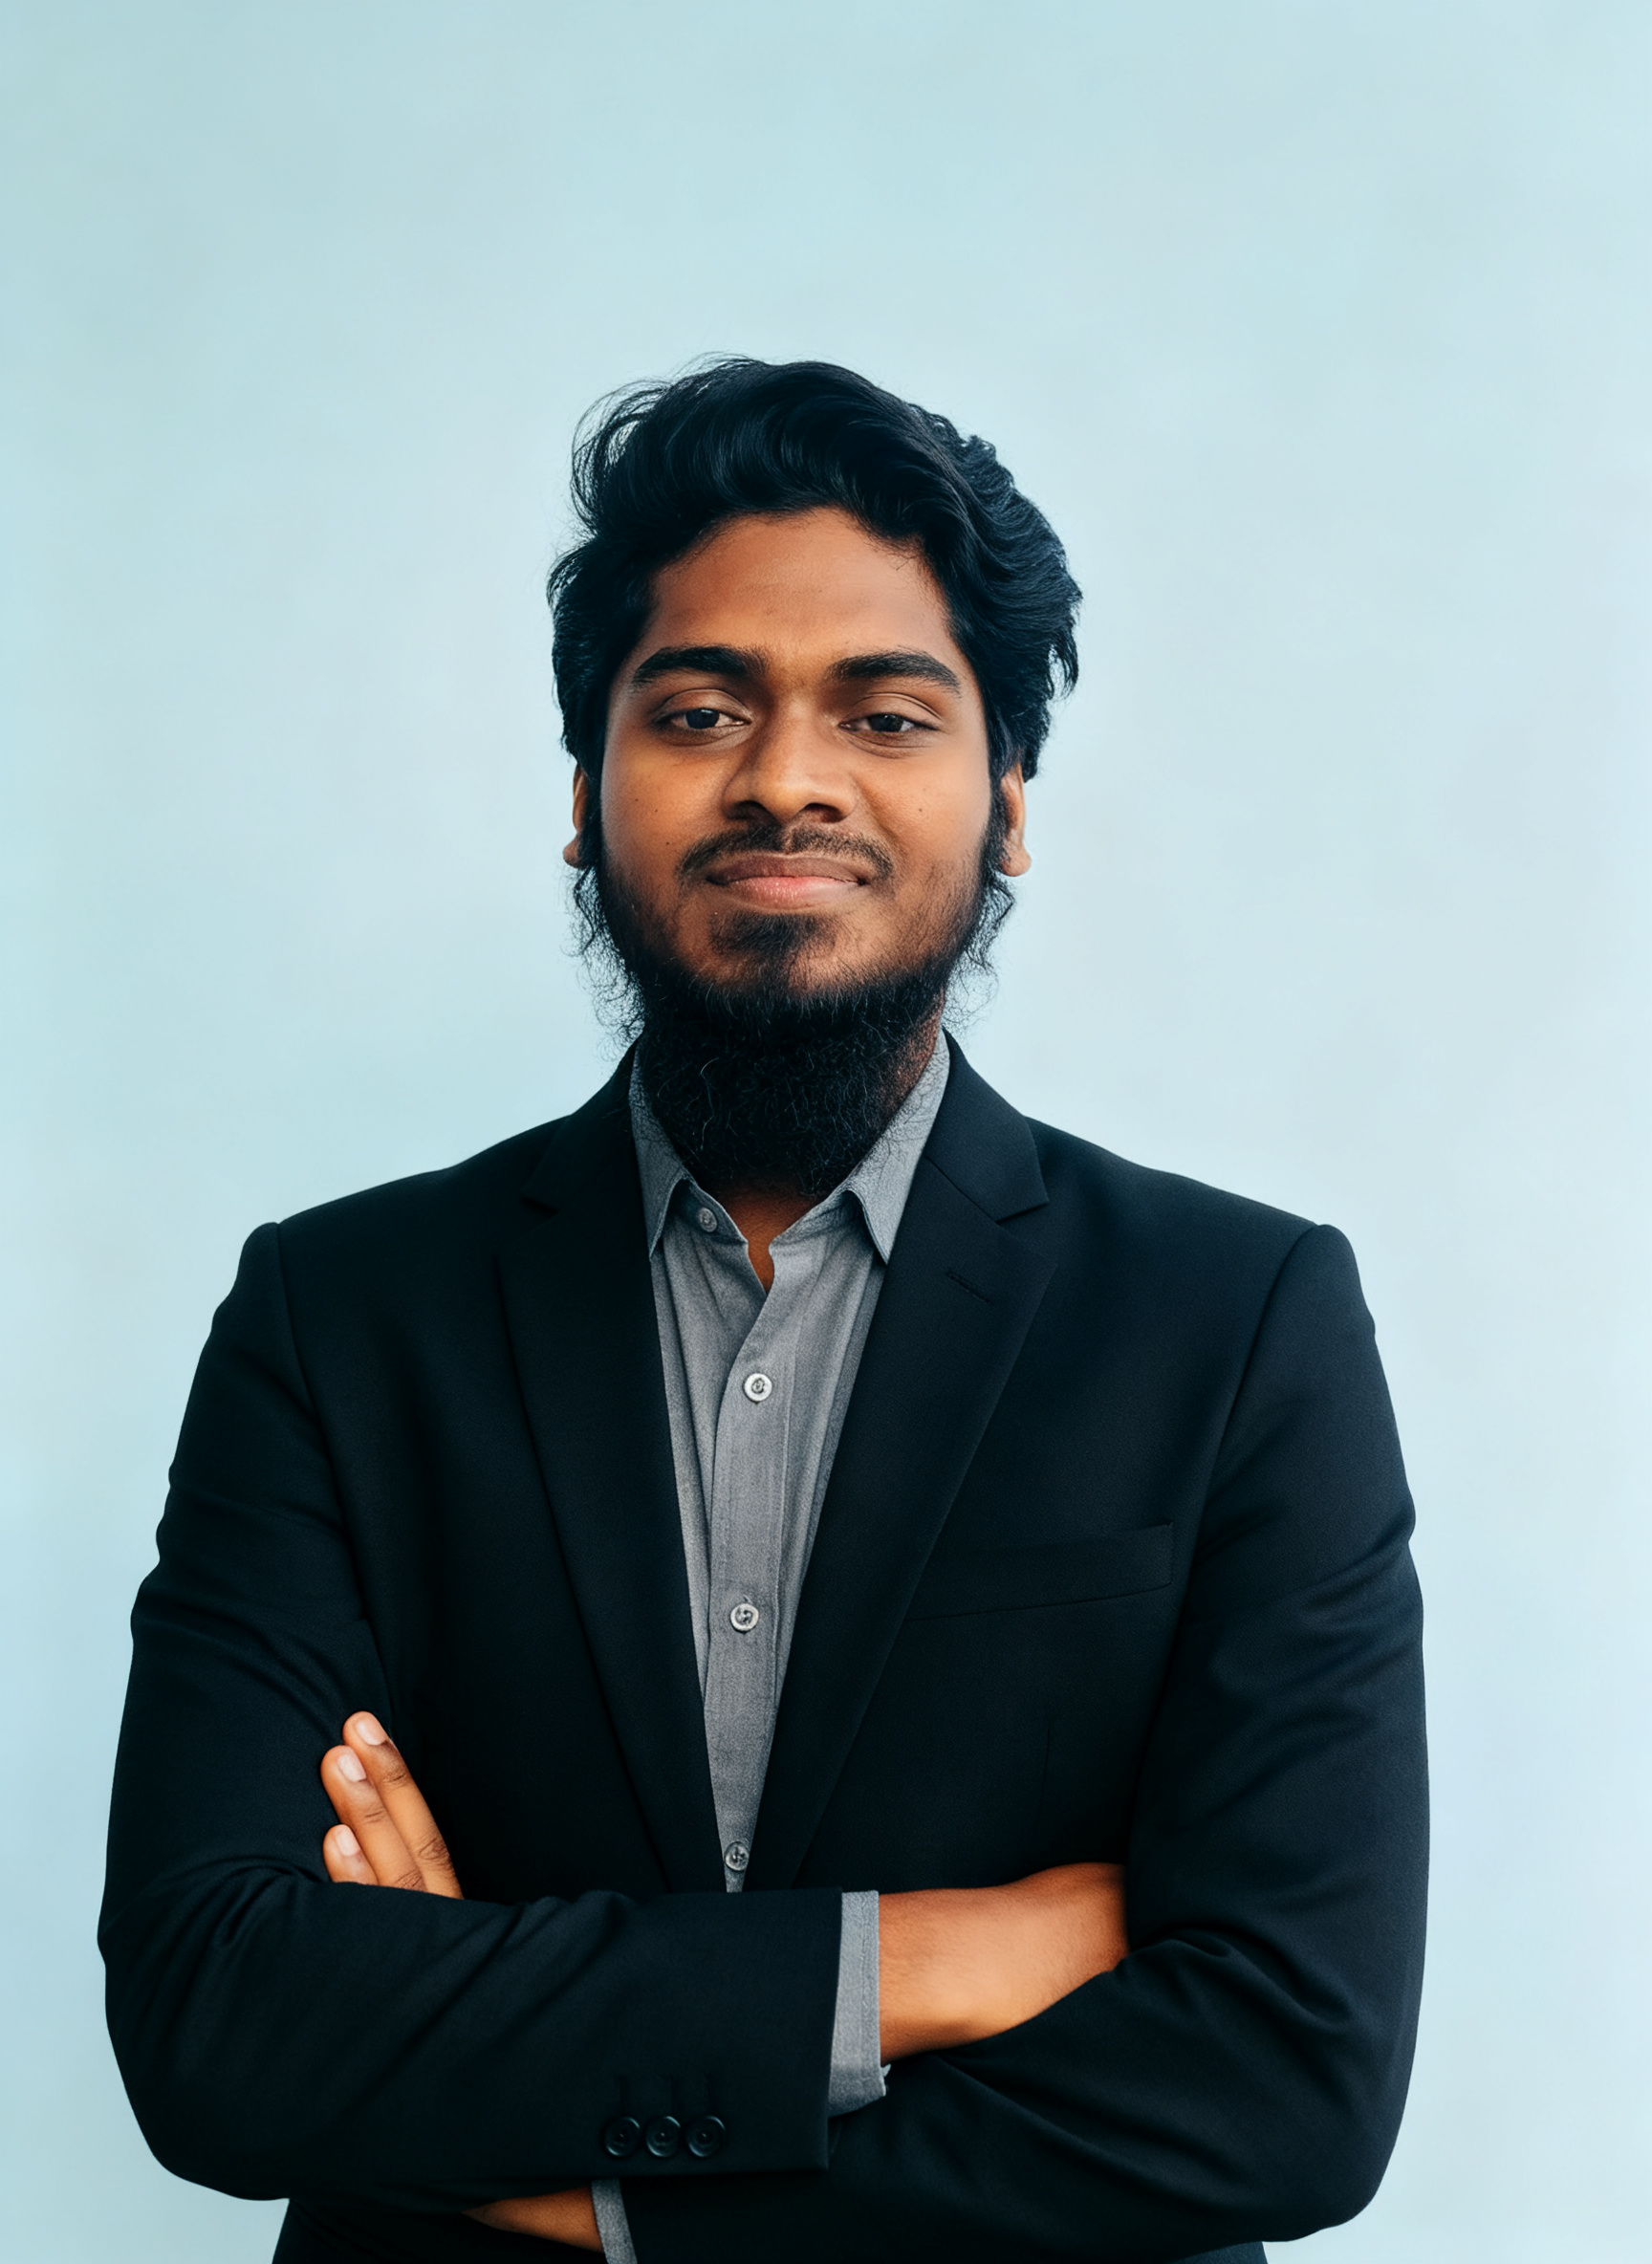
\includegraphics[width=2.6cm]{samim.jpg}};
      \end{tikzpicture}%
    }%
  }%
}

%----------HEADING----------
\begin{center}
    {\Huge \scshape \textbf{SAMIM REZA}} \\[4pt]
    \textcolor{lightgray}{
        \faPhone\ +8801747773315 \quad
        \faEnvelope\ \href{mailto:samimreza2111@gmail.com}{samimreza2111@gmail.com} \quad
        \faMapMarker\ Dhaka, Bangladesh \\[2pt]
        \faLinkedin\ \href{https://linkedin.com/in/samim-reza}{linkedin.com/in/samim-reza} \quad
        \faGithub\ \href{https://github.com/samim-reza}{github.com/samim-reza} \quad
        \faGlobe\ \href{https://samimreza.me}{samimreza.me}}
\end{center}

%-----------EDUCATION-----------
\section{Education}

\vspace{0.2cm}

\textbf{Green University of Bangladesh} \hfill \textcolor{lightgray}{2022 -- 2025}\\
B.Sc. in Computer Science and Engineering \textcolor{lightgray}{(CGPA: 3.80/4.00)}

\vspace{0.2cm}
\textbf{Government Bangabandhu College} \hfill \textcolor{lightgray}{2017 -- 2019}\\
Higher Secondary Certificate \textcolor{lightgray}{(GPA: 4.75/5.00)}

\vspace{0.2cm}
\textbf{S. M. Model Govt. High School} \hfill \textcolor{lightgray}{2012 -- 2017}\\
Secondary School Certificate \textcolor{lightgray}{(GPA: 5.00/5.00)}

%-----------WORK EXPERIENCE-----------
\section{Work Experience}
\vspace{0.2cm}
\textbf{Lead Engineer} | \textit{SolaneCode, New York} \hfill [\href{https://remitjob.com/}{Live Platform}] \textcolor{lightgray}{May 2026 -- Present}
\begin{itemize}[noitemsep, topsep=0pt]
    \item Lead engineering for a live restaurant AI phone receptionist SaaS sold in New York
    \item Built and own the AI voice workflow, frontend, backend, QA, CRM, menu, kitchen flow, and reporting systems
\end{itemize}
\vspace{0.2cm}
\textbf{Machine Learning Engineer} | \textit{Brandifies} \hfill \textcolor{lightgray}{Dec 2025 -- Present}
\begin{itemize}[noitemsep, topsep=0pt]
    \item Built end-to-end ML pipelines, Fine-tuned LLMs and implemented RAG-based chatbot systems
    \item Developed predictive models using boosting algorithms
\end{itemize}
\vspace{0.2cm}
\textbf{Robotics Engineer Intern} | \textit{RoboTech Valley} \hfill \textcolor{lightgray}{Jul -- Sept 2025}
\begin{itemize}[noitemsep, topsep=0pt]
    \item Designed robotics modules using embedded systems and ROS for autonomous navigation
\end{itemize}
\vspace{0.2cm}
\textbf{Teaching Assistant} | \textit{Green University of Bangladesh} \hfill \textcolor{lightgray}{May -- Aug 2025}
\begin{itemize}[noitemsep, topsep=0pt]
    \item Conducted demo classes on C Programming and Data Structures
    \item Evaluated exam scripts and prepared grade sheets
\end{itemize}
\vspace{0.2cm}
\textbf{Programming Trainer} | \textit{Green University of Bangladesh} \hfill \textcolor{lightgray}{Jan -- Dec 2025}
\begin{itemize}[noitemsep, topsep=0pt]
    \item Trained students for competitive programming through weekly problem-solving sessions
\end{itemize}
\vspace{0.2cm}
\textbf{Mentor} | \textit{University Mentorship Program} \hfill \textcolor{lightgray}{Jun 2023 -- Aug 2025}
\begin{itemize}[noitemsep, topsep=0pt]
    \item Mentored first-year students in programming fundamentals and professional tools
\end{itemize}

%-----------RESEARCH-----------
\section{Research}
\begin{itemize}[noitemsep, topsep=0pt]
\vspace{0.2cm}
    \item \textbf{Edge Detection for Smoke-Degraded Images using Fractional Derivative} (Published, 2026) -- Proposed a fractional calculus-based edge detection operator achieving robust boundary extraction under smoke and haze degradation conditions
    \vspace{0.2cm}
    \item \textbf{Denoising Diffusion Probabilistic Models} -- Integrating edge detection for enhanced image generation
    \vspace{0.2cm}
    \item \textbf{Federated Learning} -- Adaptive client selection algorithms for optimal convergence
\end{itemize}

% \resumeProjectHeading
% {Human-in-the-Loop ML}{}
% \resumeItemListStart
% \resumeItem{Survey on HITL approaches in modern ML systems.}
% \resumeItemListEnd

%-----------TECHNICAL SKILLS-----------
\section{Technical Skills}
\small{
\textbf{Languages}: C, C++, Python, Java, JavaScript \\
\vspace{0.2cm}
\textbf{AI/ML}: PyTorch, TensorFlow, Scikit-learn, LangChain, VectorDB, RAG, LLM, Roboflow \\
\vspace{0.2cm}
\textbf{Voice AI}: OpenAI Realtime, Twilio Media Streams, tool-calling agents, Chroma-backed RAG \\
\vspace{0.2cm}
\textbf{Web/Backend}: Django, FastAPI, Next.js, React, REST APIs, PostgreSQL, MySQL, PWA \\
\vspace{0.2cm}
\textbf{Tools \& Platforms}: Git, Docker, Celery, Redis, Twilio, Stripe, Meta Graph API, Linux, LaTeX, Supabase, Render, Arduino, Raspberry Pi, Jetson, ESP32, Azure, Digital Ocean
}

%-----------FEATURED PROJECTS-----------
\section{Featured Projects}

\vspace{0.2cm}
\textbf{Personal AI Assistant} --- LLM, RAG, LangChain \hfill [\href{https://samimreza.me/chat}{Live}] $|$ [\href{https://github.com/samim-reza/MyChatBot}{GitHub}]
\begin{itemize}[noitemsep, topsep=0pt]
    \item Built an LLM-powered chatbot with retrieval-augmented generation for personalized assistance, deployed at samimreza.me/chat
\end{itemize}

\vspace{0.2cm}
\textbf{TrueDoc} --- Django, React, DRF, SimpleJWT, PostgreSQL, QR \hfill [\href{https://github.com/samim-reza/TrueDoc}{GitHub}]
\begin{itemize}[noitemsep, topsep=0pt]
    \item SaaS for digital document attestation in Bangladesh with QR-backed verification, role-based access (citizen/verifier/org), JWT auth, and BDT payment model
\end{itemize}

\vspace{0.2cm}
\textbf{GoUp} --- Django, Celery, Redis, Meta Graph API, Twilio \hfill [\href{https://github.com/samim-reza/GoUp}{GitHub}]
\begin{itemize}[noitemsep, topsep=0pt]
    \item For Lead Ads automation; syncs pages/forms via Meta API, webhooks, triggers SMS follow-ups Celery \& Redis
\end{itemize}

\vspace{0.2cm}
\textbf{KobitaLM} --- Bengali Poetry Generator \hfill [\href{https://huggingface.co/samim-reza/KobitaLM}{Model}] $|$ [\href{https://github.com/samim-reza/KobitaLM}{GitHub}]
\begin{itemize}[noitemsep, topsep=0pt]
    \item Fine-tuned Gemma 2 9B with LoRA and RAG for Bengali poetry generation
\end{itemize}

\vspace{0.2cm}
\textbf{WeCare Medical Service App} --- FastAPI, Qwen3-VL, PWA \hfill [\href{https://github.com/samim-reza/FutureBuilders2025_GreenU_Tensors}{GitHub}]
\begin{itemize}[noitemsep, topsep=0pt]
    \item Developed an offline-first PWA for rural healthcare with AI-assisted triage capabilities
\end{itemize}

\vspace{0.2cm}
\textbf{Cirrhosis Outcome Prediction} --- XGBoost, LightGBM, CatBoost \hfill \textcolor{lightgray}{BAIC 2025}
\begin{itemize}[noitemsep, topsep=0pt]
    \item Built an ensemble ML classifier with 55 engineered features, achieving 14.5\% accuracy gain
\end{itemize}

\vspace{0.2cm}
\textbf{Hasib Academic System} --- Django, PostgreSQL, Render, Gunicorn \hfill [\href{https://hasibislamicacademy.github.io/}{Live}] $|$ [\href{https://github.com/samim-reza/Hasib_School}{GitHub}]
\begin{itemize}[noitemsep, topsep=0pt]
    \item A production-ready Django application for school workflows including admissions, student attendance, notices, teacher accounts, and finance tracking with PDF export. Tailored for Bangla-speaking users
\end{itemize}

\vspace{0.2cm}
\textbf{Union Ledger} --- Django, PostgreSQL, Render \hfill [\href{https://samim-reza.github.io/union}{Live}] $|$ [\href{https://github.com/samim-reza/union}{GitHub}]
\begin{itemize}[noitemsep, topsep=0pt]
    \item Built a collaborative financial tracking web app with consensus-based voting for deposits, loans, repayments, and investments
\end{itemize}

\vspace{0.2cm}
\textbf{Mars Rover} --- ROS, Embedded Systems \hfill [\href{https://github.com/samim-reza/Rover-robot}{GitHub}]
\begin{itemize}[noitemsep, topsep=0pt]
    \item Developed a ROS-based autonomous navigation system for Mars rover simulation
\end{itemize}

%-----------COMPETITIVE PROGRAMMING-----------
\section{Competitive Programming}
\begin{itemize}[noitemsep, topsep=0pt]
    \item \textbf{Champion:} Intra Dept Programming Contest 2024
    \vspace{0.2cm}
    \item \textbf{3x ICPC Regionalist:} 2022, 2023, 2024
    \vspace{0.2cm}
    \item \textbf{Kaggle Competitor:} Active in ML competitions
    \vspace{0.2cm}
    \item \textbf{Problem Setter:} Junior Programming Contests
    \vspace{0.2cm}
    \item \textbf{Participated:} NCPC 2023, IUPC 2023/2024
\end{itemize}

%-----------ACHIEVEMENTS-----------
\section{Achievements}
\begin{itemize}[noitemsep, topsep=0pt]
    \item Vice Chancellor's Award for Academic Excellence
    \vspace{0.2cm}
    \item Champion, Inter Dept Programming Contest 2024
    \vspace{0.2cm}
    \item Secured \textbf{8th} position in BUBT Artificial Intelligence Conquest in Kaggle
    \vspace{0.2cm}
    \item National IT Quiz Competition Medalist
\end{itemize}

%-----------REFERENCES-----------
\section{References}

\begin{multicols}{2}
\textbf{Prof. Dr. Md. Saiful Azad} \\
Dean, Faculty of Science \& Engineering \\
Green University of Bangladesh \\
Email: dean@fse.green.edu.bd \\
Mobile: +880 1747-230418

\columnbreak

% \vspace{6pt}
\textbf{Ms. Umme Ruman} \\
Assistant Professor \\
Green University of Bangladesh \\
Email: ruman@cse.green.edu.bd \\
Mobile: +880 1799-089667
\end{multicols}

\end{document}
